\section{DCGAN}
The \gls{DCGAN} architecture was a big step for \acp{GAN} when it was introduced, it defined a set of recommendations for building networks that would be more stable and scalable, by fully leveraging the power of convolutional layers in both generator and discriminator \cite{dcgan2015}. The architecture of the \gls{DCGAN} was used as a basis for all following experiments in this document.

The goal of the tests in this section was to try and find what properties of the \gls{DCGAN} were relevant, what configurations could be used to tackle different situations, and to question the validity of using transposed convolutions has a way of upscaling the latent vector to the full resolution of the image, since it can produce artifacts \cite{deconvolutionArtifacts2016} and it is being replaced in recent approaches (e.g. \cite{styleGAN2018}) by more conventional upsampling techniques followed by a simple dimension preserving convolution.

\subsection{MNIST}
Training the \gls{DCGAN} on the \gls{MNIST} dataset produced the results seen in \autoref{fig:dcgan_mnist_metrics}.\begin{figure}[hbt]
    \centering
    \caption{Metrics when training a DCGAN on MNIST}
    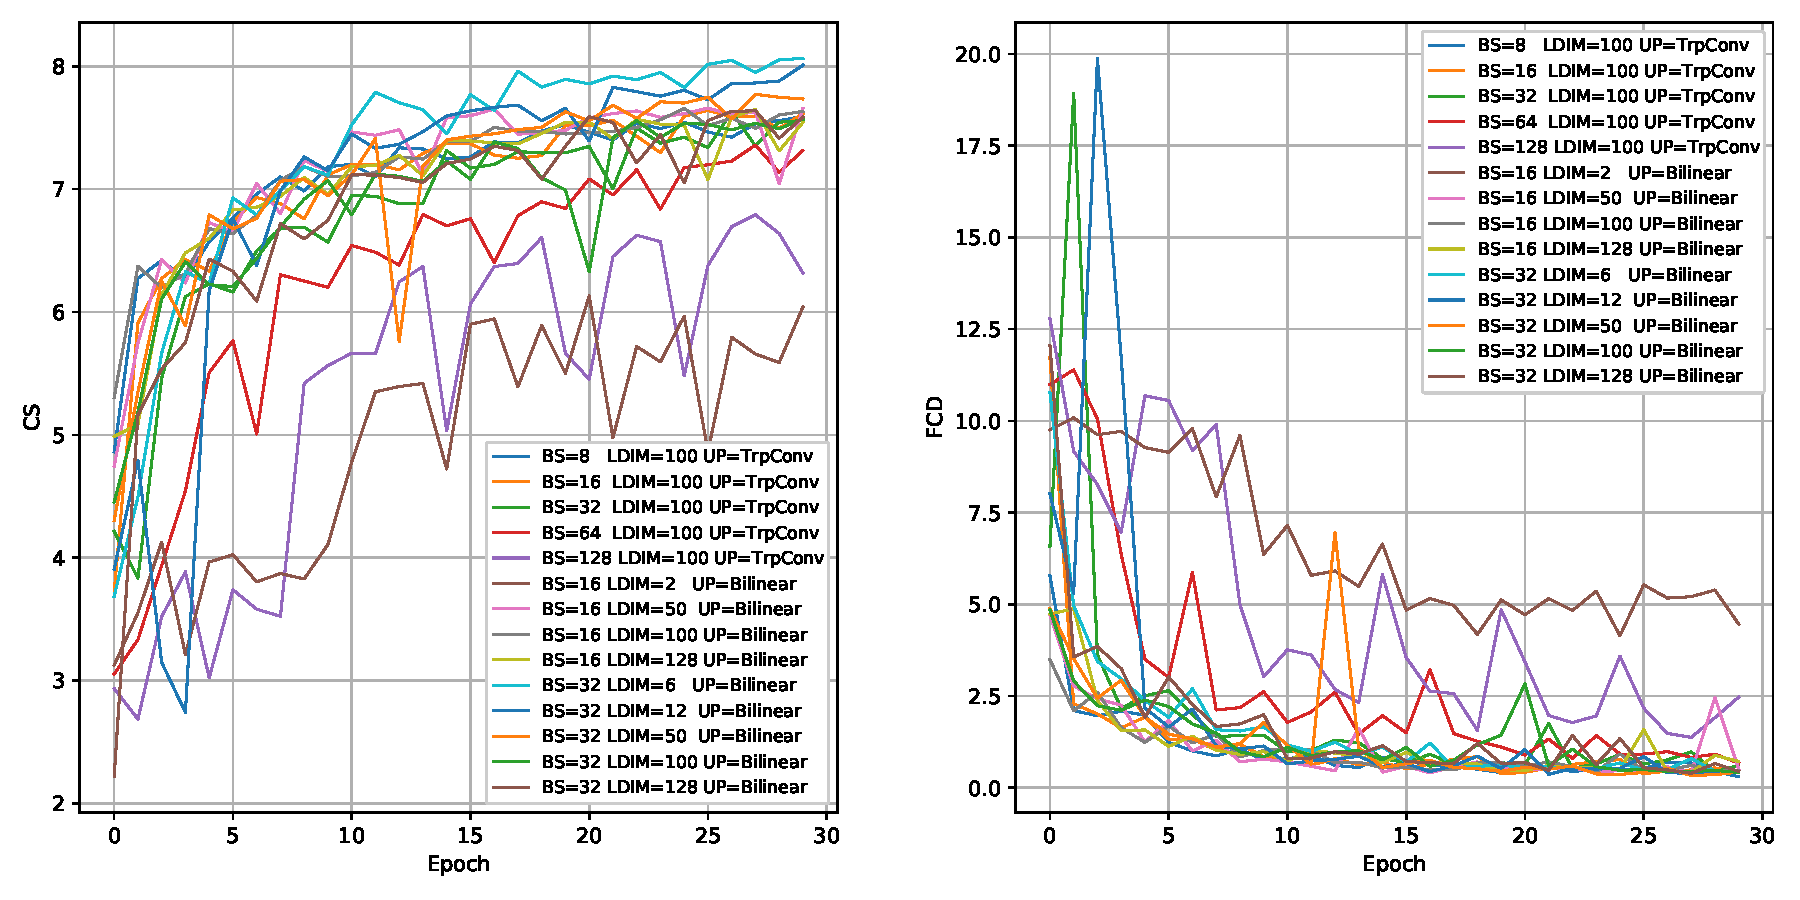
\includegraphics[width=0.9\textwidth]{chapters/Experiments/DCGAN/mnist_metrics.pdf}
    \fonte{From the author (2021)}
    \label{fig:dcgan_mnist_metrics}
\end{figure}

There are a couple of things that can be observed in these results. First, observe how the number of dimensions in the latent space does not seem to be very relevant, unless it becomes too small, as seen for the case of \texttt{LDIM=2}, which produced the worst results. This makes sense since it is harder for the generator to learn a map from the smaller space to all possible images, in other words, it's capacity is too small to produce the complexity in the data.

The effect of this can be seen in \autoref{fig:dcgan_mnist_ldim2}, these are samples produced by the generator with only two dimensions of latent space. The samples were chosen in a training epoch where it is particularly clear that the generator is producing some relatively good samples, but it suffers to map the small volume of the latent space into all possible digits, resulting in mode collapse.
\begin{figure}[hbt]
    \centering
    \caption{Samples taken from a DCGAN with low dimensions of latent space}
    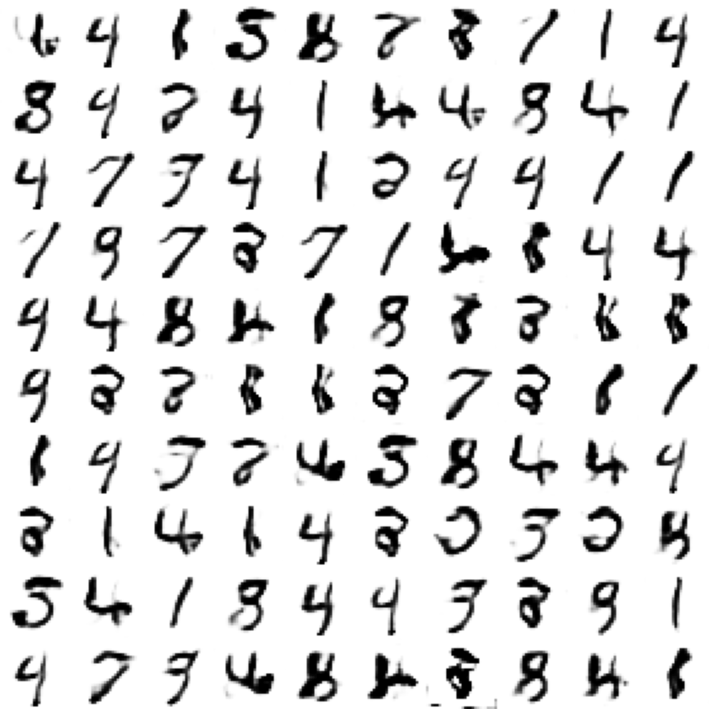
\includegraphics[width=0.5\textwidth]{chapters/Experiments/DCGAN/mnist_ldim2.png}
    \fonte{From the author (2021)}
    \label{fig:dcgan_mnist_ldim2}
\end{figure}

But note that by just raising the number of dimensions from 2 to 6 is already enough to fix this problem, after that, the number of increased dimensions has little effect, since the generator already has all the capacity it needs to represent the simple data from the \gls{MNIST} dataset.

The results in \autoref{fig:dcgan_mnist_metrics} cannot give a definitive answer about the influence of the batch size, although there is some indication that bigger batches may not be ideal. This is seen for the case with batch size of 128 that produced the second least favorable results, and in a lesser extent for the test with batch size of 64.

Last point of note is the effect of the upsampling technique used, to better visualize this it is helpful to group the metrics shown in \autoref{fig:dcgan_mnist_metrics} into the particular sets of interest, this approach will be used repeatedly for the rest of this document. \autoref{fig:dcgan_mnist_upsampling} highlights the results per type of upsampling used.
\begin{figure}[hbt]
    \centering
    \caption{Effects of upsampling when training a DCGAN on MNIST}
    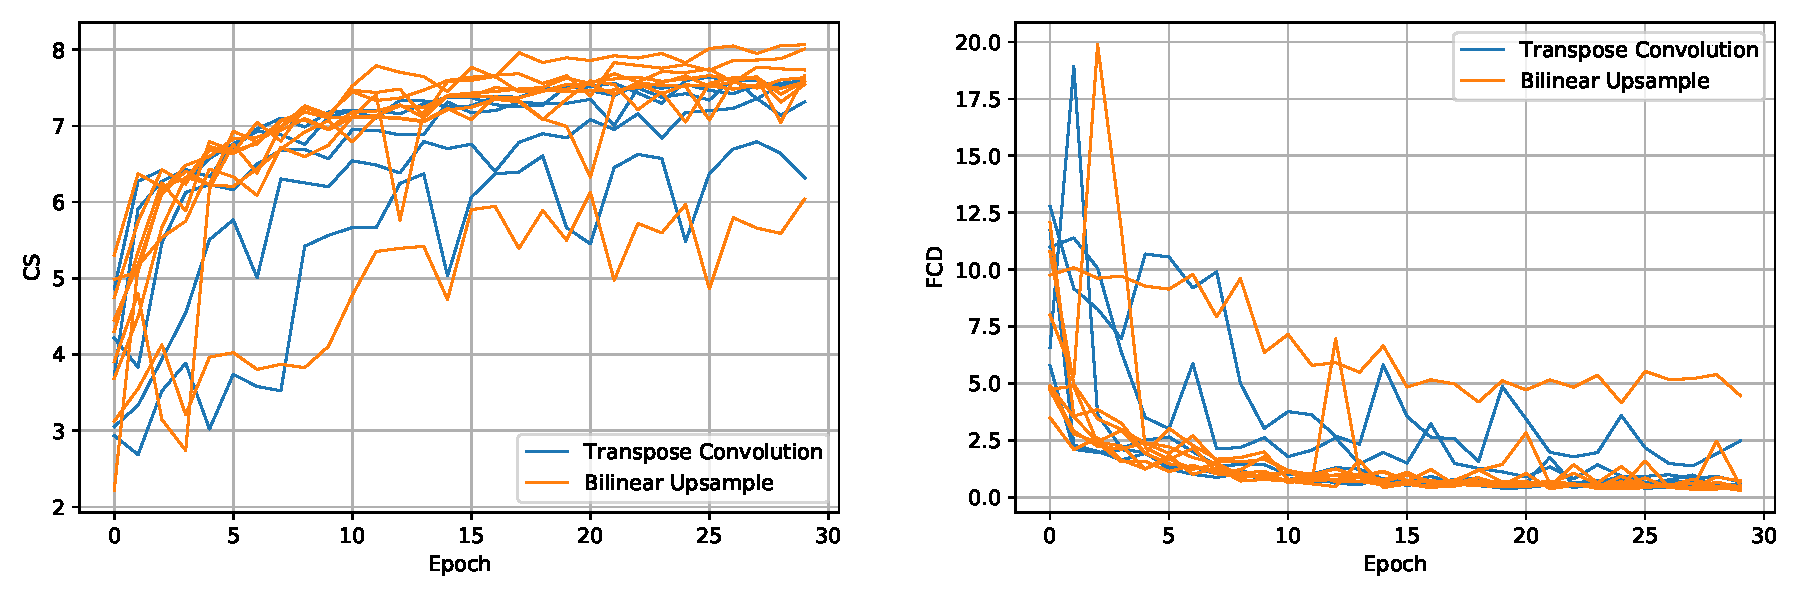
\includegraphics[width=\textwidth]{chapters/Experiments/DCGAN/mnist_upsampling.pdf}
    \fonte{From the author (2021)}
    \label{fig:dcgan_mnist_upsampling}
\end{figure}

It can be seen by this figure that the bilinear upsampling technique generally performs better than transposed convolutions in the case of \gls{MNIST}, as later results will show, this does not imply that it will always be the case.

\autoref{fig:dcgan_mnist_samples} shows samples produced by the best model experimented in these tests, with configuration (\texttt{BS=32 LDIM=12 UP=Bilinear}).
\begin{figure}[hbt]
    \centering
    \caption{Samples when training a DCGAN on MNIST}
    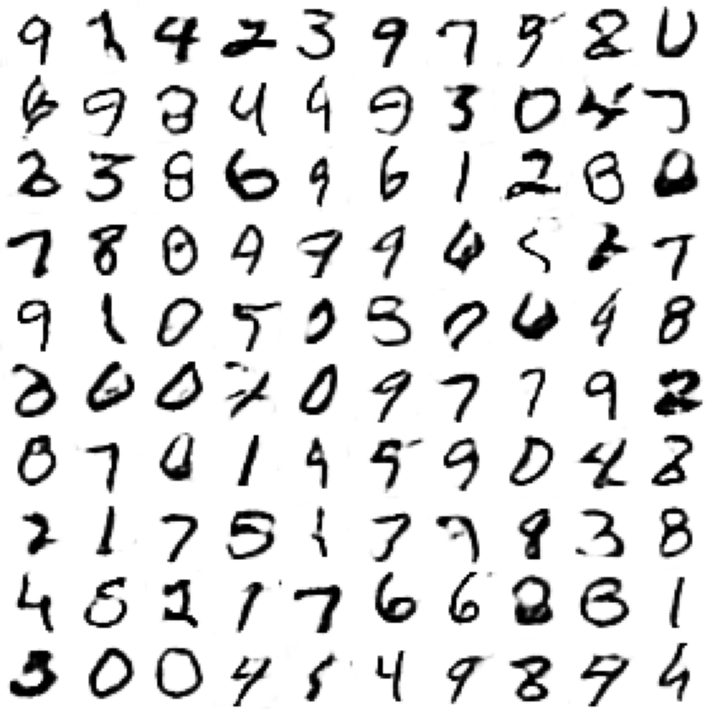
\includegraphics[width=0.5\textwidth]{chapters/Experiments/DCGAN/mnist_samples.png}
    \fonte{From the author (2021)}
    \label{fig:dcgan_mnist_samples}
\end{figure}


\subsection{Fashion MNIST}
Training the \gls{DCGAN} on the Fashion MNIST dataset produced the results seen in \autoref{fig:dcgan_fashion_metrics}.
\begin{figure}[hbt]
    \centering
    \caption{Metrics when training a DCGAN on Fashion MNIST}
    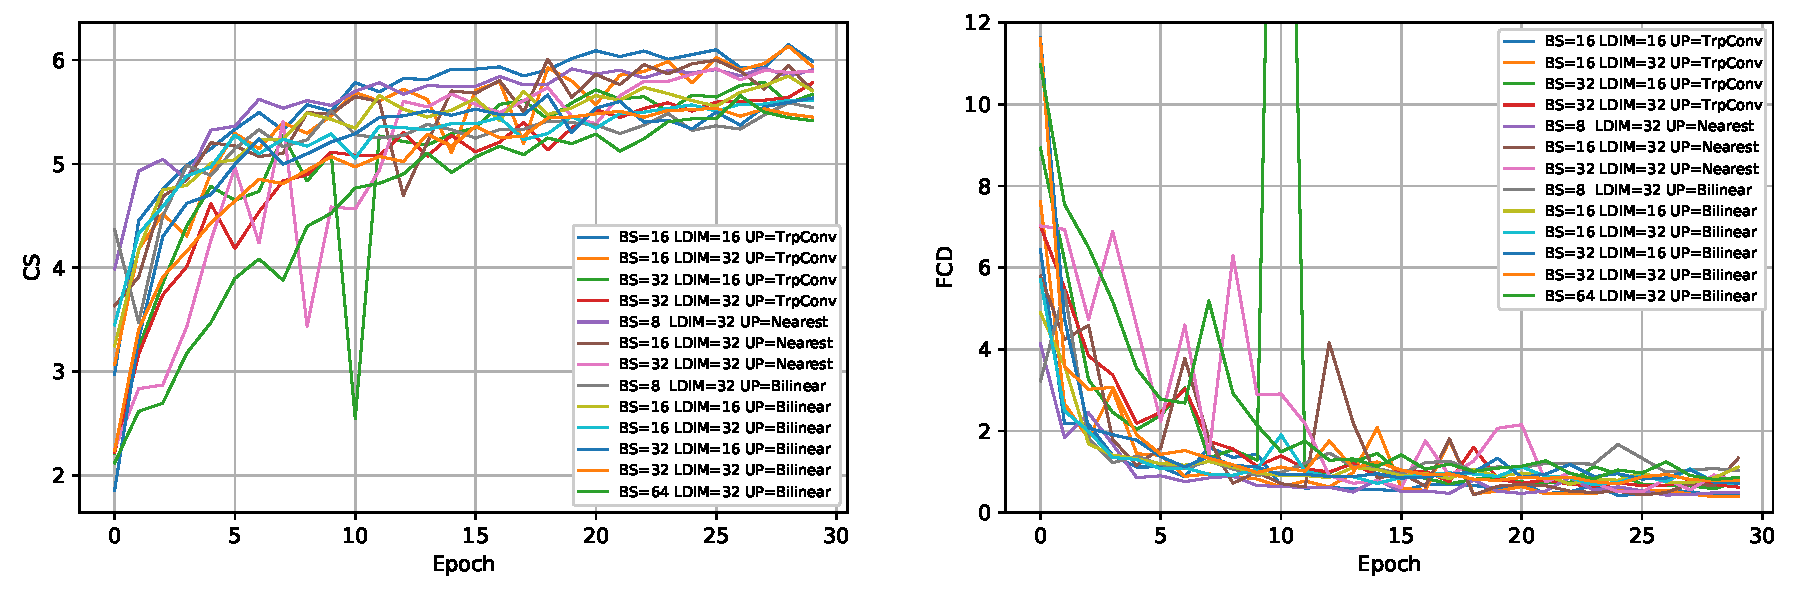
\includegraphics[width=\textwidth]{chapters/Experiments/DCGAN/fashion_metrics.pdf}
    \fonte{From the author (2021)}
    \label{fig:dcgan_fashion_metrics}
\end{figure}

Again the use of bigger batches has produced weaker results, with the case for a batch size of 64 producing the least favorable overall results between all tests. This may be for the fact that smaller batch sizes have more updates per epoch since they divide the dataset into more batches and each batch is a parameter update. However, at least for the case of the batch size of 128 seen in \autoref{fig:dcgan_mnist_metrics}, bigger batches seem to have more difficulty to step beyond a certain point. It may be that bigger batches would produce better results given more epochs of training, and they are a small amount faster to calculate per epoch in relation to smaller batches, but for the rest of the tests they were not evaluated more deeply.

One thing to note is the extreme jump seen on test (\texttt{BS=32 LDIM=16 UP=TrpConv}), this can be seen to a smaller extent in many cases throughout the following experiments, but this was the most extreme one. It is not clear why this happens, the author's hypothesis is that the generator stepped into a particular steep region of the loss surface, but was quickly pointed in the right direction by the larger gradients of the discriminator in the next updates.

Again, by highlighting the use of the upsampling techniques it is possible to obtain the results seen in \autoref{fig:dcgan_fashion_upsampling}. In this case, the transposed convolutions showed the best results, while bilinear upsampling had the least favorable overall. The nearest neighbour interpolation was also tested in this case and here it also performed better than bilinear.
\begin{figure}[hbt]
    \centering
    \caption{Effects of upsampling when training a DCGAN on Fashion MNIST}
    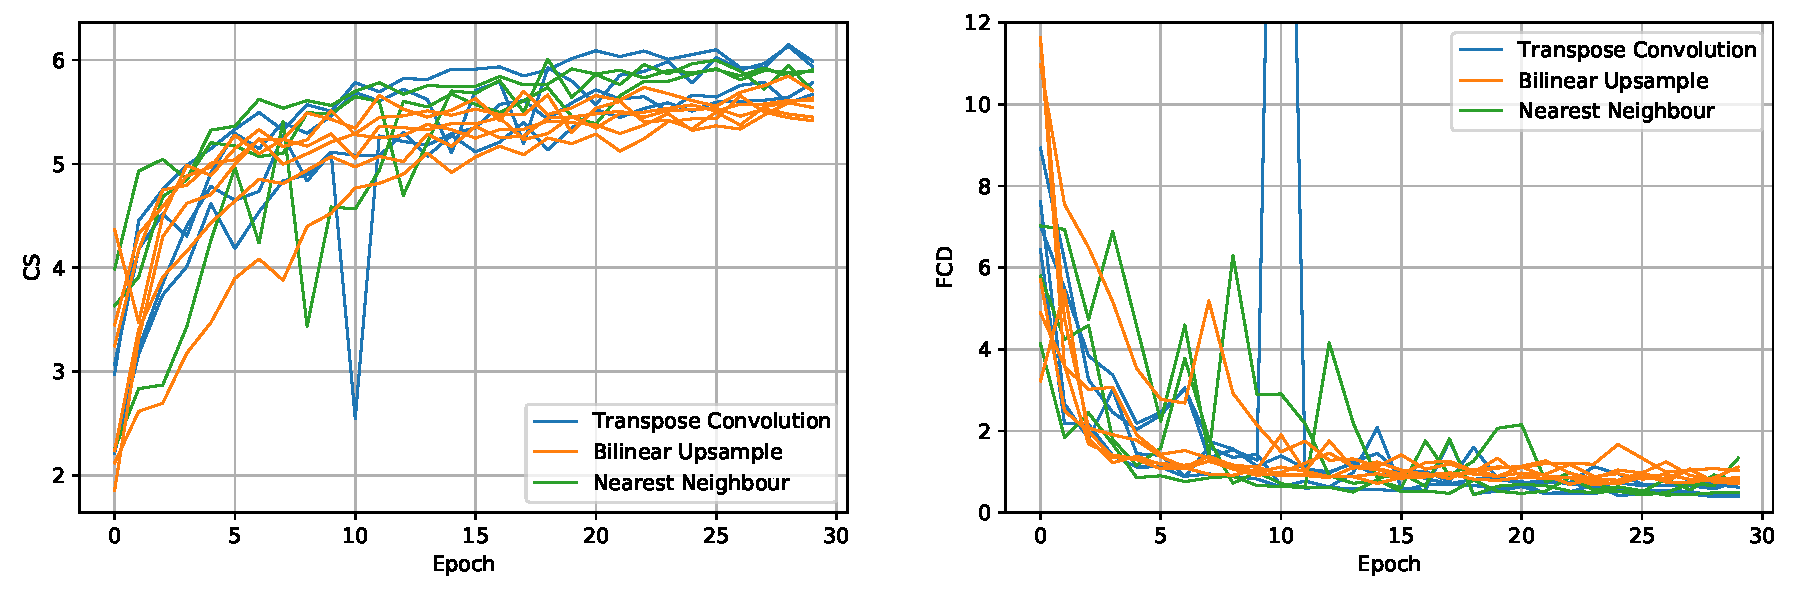
\includegraphics[width=\textwidth]{chapters/Experiments/DCGAN/fashion_upsampling.pdf}
    \fonte{From the author (2021)}
    \label{fig:dcgan_fashion_upsampling}
\end{figure}

Lastly, the samples from the lowest \gls{FCD} obtained by the test (\texttt{BS=16 LDIM=32 UP=TrpConv}) can be seen in \autoref{fig:dcgan_fashion_samples}. Note how the generator does not have a good sense of symmetry, producing shirts with long sleeves in a single arm. This is a very common occurrence in \acp{GAN}, even modern models will suffer from this; for example, \acp{GAN} can produce faces where the eyes do not have the same color, or place different earrings in each ear \cite{gan_asymmetry2018}.
\begin{figure}[hbt]
    \centering
    \caption{Samples when training a DCGAN on Fashion MNIST}
    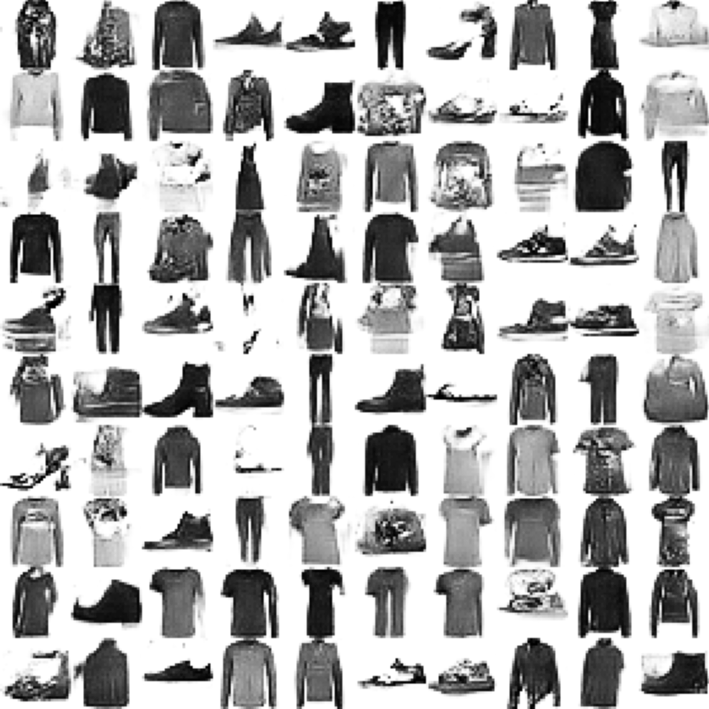
\includegraphics[width=0.5\textwidth]{chapters/Experiments/DCGAN/fashion_samples.png}
    \fonte{From the author (2021)}
    \label{fig:dcgan_fashion_samples}
\end{figure}


\subsection{CIFAR-10}
\autoref{fig:dcgan_cifar_metrics} shows the results of training the \gls{DCGAN} on the \gls{CIFAR}-10 dataset. One thing to note here is how both the \gls{CS} and \gls{FCD} metrics show weaker results when compared to the previous results.
\begin{figure}[hbt]
    \centering
    \caption{Metrics when training a DCGAN on CIFAR-10}
    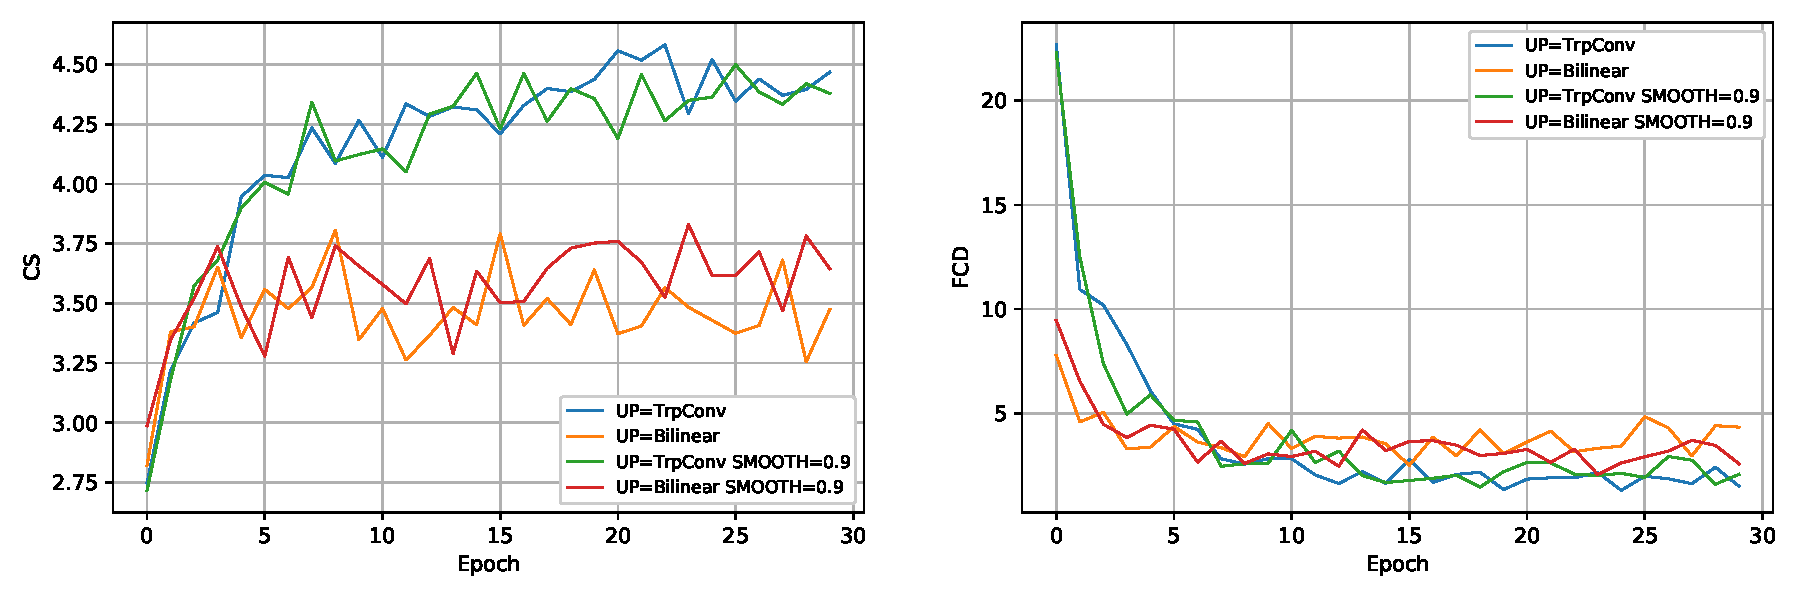
\includegraphics[width=\textwidth]{chapters/Experiments/DCGAN/cifar_metrics.pdf}
    \fonte{From the author (2021)}
    \label{fig:dcgan_cifar_metrics}
\end{figure}

When making the experiments, it was found that the \gls{CIFAR}-10 dataset is considerably harder than the other datasets, even when compared with the CelebA and Flowers datasets. The author's hypothesis is that this is due to the relatively low number of images for each class in \gls{CIFAR}-10, (only $6000$ for each), and that the classes are significantly different from each other, making it very hard for the generator to learn the details in all of them.

Recall that the classes in \gls{CIFAR}-10 are: \texttt{airplane}, \texttt{automobile}, \texttt{bird}, \texttt{cat}, \texttt{deer}, \texttt{dog}, \texttt{frog}, \texttt{horse}, \texttt{ship} and \texttt{truck}. These images are significantly more varied than the other datasets used, even the dataset of human faces, CelebA, can later be seen to be relatively homogeneous.

With these results it is possible to see once again a clear difference between upscaling techniques. This time, in accordance with what was seen for Fashion MNIST, the transposed convolution gives the best results. In these tests it was also experimented the use of one sided label smoothing, although the results still do not show any significant difference that allows for making conclusions.

One important thing to note in all the tests on CIFAR made for this document, is the fact that the momentum term of the Adam optimizer (\gls{beta_1}) had a negative impact on the convergence of the models. For \gls{MNIST} and Fashion MNIST this term was kept at the common value of $0.9$ without any problems, however this would result in incomprehensible images and no sort of convergence when training on \gls{CIFAR}-10, to avoid this, \gls{beta_1} was kept at zero.

The samples produced for the best overall \gls{FCD} in the test (\texttt{UP=TrpConv}) are shown in \autoref{fig:dcgan_cifar_samples}. Note how it is possible to see a hint of the \gls{CIFAR}-10 classes in these images, but nothing can be pointed out as a completely sensible real world object.
\begin{figure}[hbt]
    \centering
    \caption{Samples when training a DCGAN on CIFAR-10}
    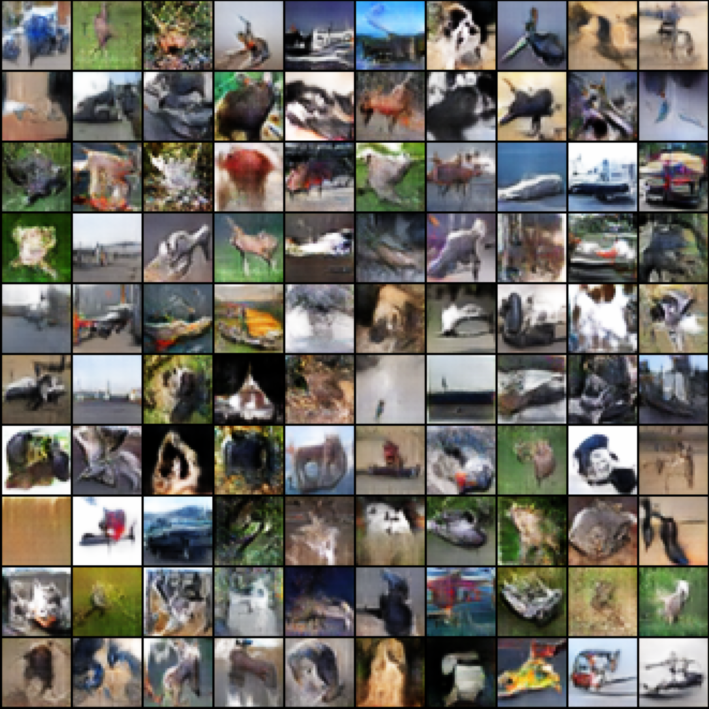
\includegraphics[width=0.5\textwidth]{chapters/Experiments/DCGAN/cifar_samples.png}
    \fonte{From the author (2021)}
    \label{fig:dcgan_cifar_samples}
\end{figure}
